\documentclass{article}
\usepackage{tikz}



\begin{document}

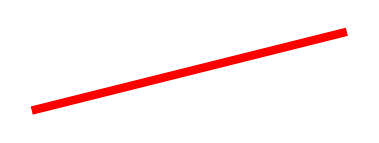
\begin{tikzpicture}[line width = 3pt, color = red]
  \draw (0,0) -- (4,1);
\end{tikzpicture}

Hola mundo

\tikz{
  \draw[line width = 4pt] (0,0) -- (4,1);
  \draw[color=red] (0,0) -- (4,-1); 
}

\section{Especificaciòn de puntos}

\begin{center}
  \begin{tikzpicture}
    \draw (5,5) circle (1pt);
    \draw (1,1,1) circle (3pt);
  \end{tikzpicture}
\end{center}

\begin{center}
  \begin{tikzpicture}
    \draw (0,0) -- (45:2);
  \end{tikzpicture}
\end{center}

\begin{center}
  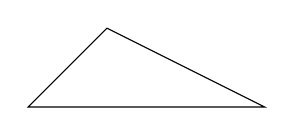
\begin{tikzpicture}
    \draw (1,1) -- ++ (1,1) -- ++ (2,-1) -- cycle;
  \end{tikzpicture}
\end{center}

\section{Acciones con caminos o path}
\begin{center}
  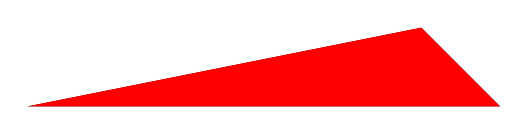
\begin{tikzpicture}
    \path[fill] (0,0) -- (5,1) -- ++ (1,-1);
    \path[fill=red] (0,0) -- (5,1) -- ++ (1,-1);
  \end{tikzpicture}
\end{center}

\section{Opciones de comandos tikz}

\begin{center}
  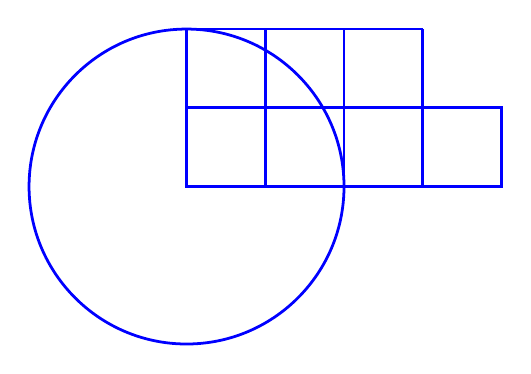
\begin{tikzpicture}[line width = 1pt, color = blue]
    \draw (0,0) rectangle (4,1);
    \draw (0,0) circle (2);
    \draw (0,0) grid (3,2);
  \end{tikzpicture}
\end{center}

\section{Sintaxis especiales con nodo}
\begin{center}
  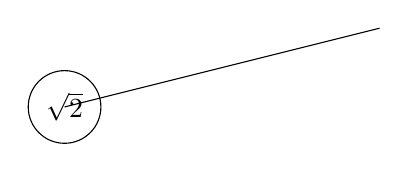
\begin{tikzpicture}
    \draw (0,0) node[draw, circle] {$\sqrt{2}$} -- (4,1);
  \end{tikzpicture}
\end{center}

\begin{center}
  \begin{tikzpicture}
    \draw (0,0) node[draw]{A}-- (4,1);
  \end{tikzpicture}
\end{center}

\section{Entorno scope}
\begin{center}
  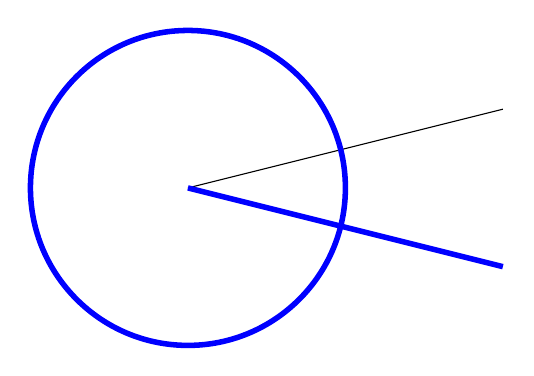
\begin{tikzpicture}
    \draw (0,0) -- (4,1);
    \begin{scope}[color = blue, line width = 2pt]
      \draw (0,0) -- (4,-1);
      \draw (0,0) circle (2);
    \end{scope}
  \end{tikzpicture}
\end{center}

\section{Especificaciòn de coordenadas}
\begin{center}
  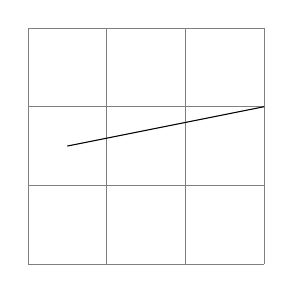
\begin{tikzpicture}
    \draw[help lines] (0,0) grid (3,3);
    \draw ([xshift=-5mm,yshift=5mm]1,1) -- (3,2);
  \end{tikzpicture}
\end{center}



\end{document}
